\section{Strategie}
Um die Ausgangslage zu verbessern, können verschiedene Ansätzte gewählt werden. In diesem Konzept wird die Möglichkeit der Exemplarfindung im Hochregallager untersucht. Sollte ein bestimmtes Exemplar verloren gehen, soll diese automatisiert im Hochregallager wiedergefunden werden. Die so vereinfachte Wiederfindung soll der Speicherbibliothek zu einer erhöhten Sicherheit bezüglich der Einlagerung der Exemplare verhelfen. Es soll bewirkt werden, dass deplatzierte Exemplare ohne grösseren personellen Aufwand wiederbeschafft werden können.

\section{Ideenbeschreibung}
Momentan fährt der Roboter nur die im System hinterlegte Position des Behälters an. Diese Fahrt wird durch die Software des Logistiksystems mitsamt des Roboters gesteuert. Neu soll die Software dieses Herstellers so erweitert werden (Siehe \ref{sec:roboterSWAnpassung}), dass der Roboter einen vordefinierten Pfad abfährt mit einem speziellen RFID Lesebehälter/Suchbehälter (Siehe \ref{sec:behaelterMitRFID}) und dabei noch Aktionen ausführt, wie die temporäre Einlagerung dieses Behälters und Zwischenlagerung des Behälters, welcher sich an der eingelagerten Stelle befand.
Würde nun ein Buch, welches von einer Bibliothek oder einem anderen Kunden bestellt wurde, nicht im entsprechenden Behälter zu finden sein, soll neu der spezielle RFID Lese-/Suchbehälter in das Hochregallager geschickt werden.


Dabei gibt es zwei Unterschiedliche Suchmodi. Als Erstes würde der Roboter mit dem Lese-/Suchbehälter in alle Gassen geschickt, wo dieser durch jede Reihe nacheinander fährt. Dabei wird jeweils vom Lese-/Suchbehälter der Vordere Behälter nach dem fehlenden Exemplar abgesucht. So kann in einer Kurzer Zeit ca. 50\% des Lagers nach dem deplatzierten Exemplar abgesucht werden. Würde nach diesem Suchvorgang die Lokalisation des Exemplares nicht erfolgreich abgeschlossen werden, würde in der Nacht die zweite Suchfunktion starten, bei welcher der Lese-/Suchbehälter im Hochregallager in der Höhe jeden dritten Platz eines äusseren bereits abgesuchten Behälters für eine kurze Zeit tauscht. Während der Lese-/Suchbehälter am äusseren Platz ist sucht er im hinteren Behälter nach dem Exemplar sowie in den dem abgesuchten Behälter direkt Benachbarten Behältern.

\subsection{Anpassungen Lagerverwaltungssoftware}
\label{sec:roboterSWAnpassung}
Für die Software der Lagerverwaltung soll die Herstellerfirma dieser Software diese um eine Schnittelle erweitern, welche es ermöglicht dem Roboter über das Netzwerk neue Fahrpositionsdaten mitzuteilen, zu welchen er anschliessend fährt. Es soll dabei möglich sein dem Roboter zu sagen, ob er einen Behälter tauschen soll oder nur an die Position fahren soll. Zudem soll die momentane Position des Roboters über diese Schnittelle abgefragt werden können. 

\subsection{Behälter mit RFID Ausrüstung}
\label{sec:behaelterMitRFID}
Die heutige RFID HF Technologie, welche bereits in der Speicherbibliothek zum Einsatz kommt ist auf ca. 1m Distanz beschränkt. Dies bedeutet, dass es nicht möglich ist alle Tags direkt vom Roboter aus zu lesen. Um alle Behälter auslesen zu können muss also der Behälter die Position eines anderen Behälters einnehmen, um den hinteren Behälter lesen zu können. Da es jedoch enorm zeitintensiv ist, jede vordere Kiste mit dem Lese-/Suchbehälter auszutauschen, sollen multiple Antennen zum Einsatzt kommen. Diese sollen so ausgerichtet werden, dass nicht nur der hintere Behälter sondern auch dessen Nachbarn ausgelesen werden können.
Die Antennen sollen gemäss Abbildung \ref{fig:antennenPositionen} ausgerichtet werden.

\begin{figure}[htb]
	\centering
	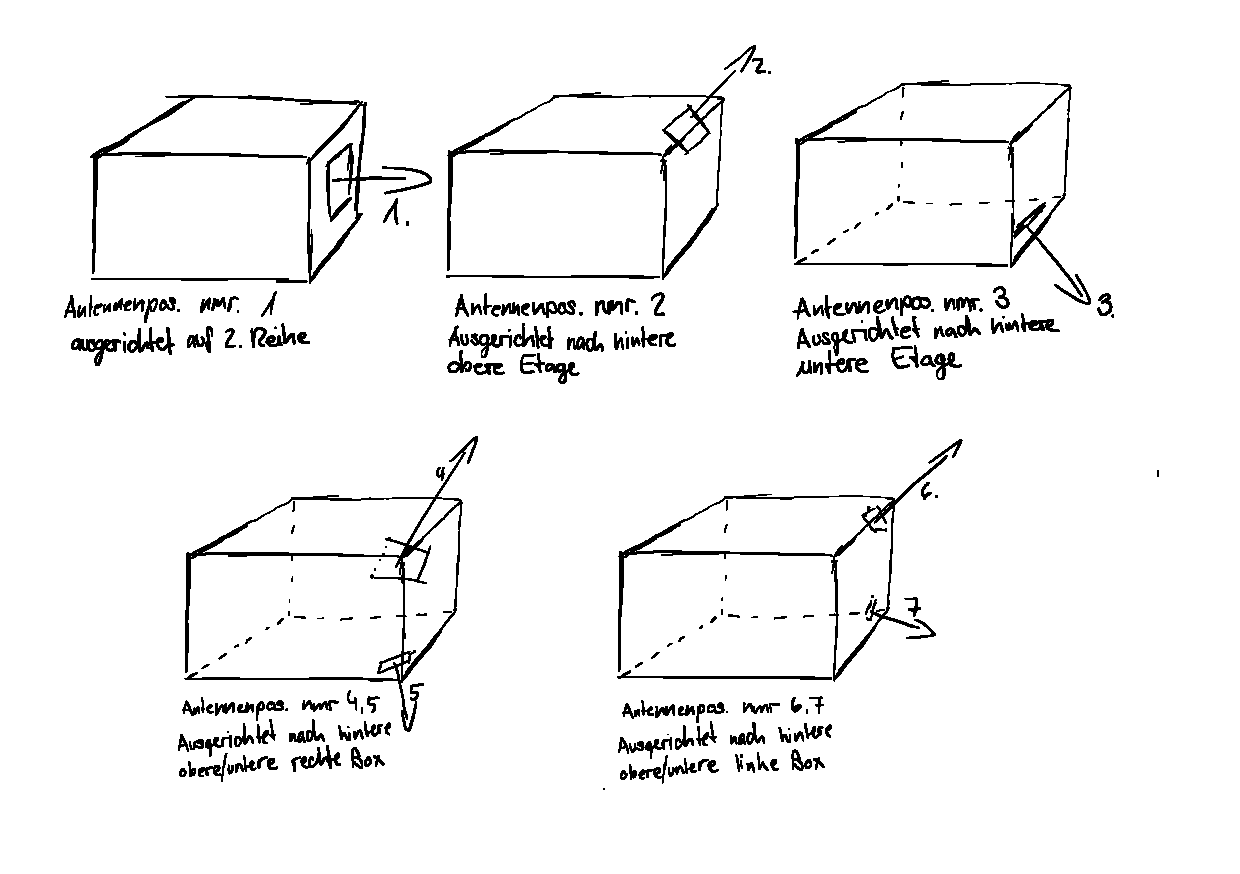
\includegraphics[keepaspectratio, width=1\textwidth]{antennen_auf_behaelter}
	\caption{Alle Antennenpositionen in einer Box für die Rechte Seite}
	\label{fig:antennenPositionen}
\end{figure}

In der Abbildung \ref{fig:distanzcalc} wird dargestellt, dass alle äusseren Behälter noch innerhalb der von HF RFID möglichen Lesedistanz von unter 1m liegen.

\begin{figure}[htb]
	\centering
	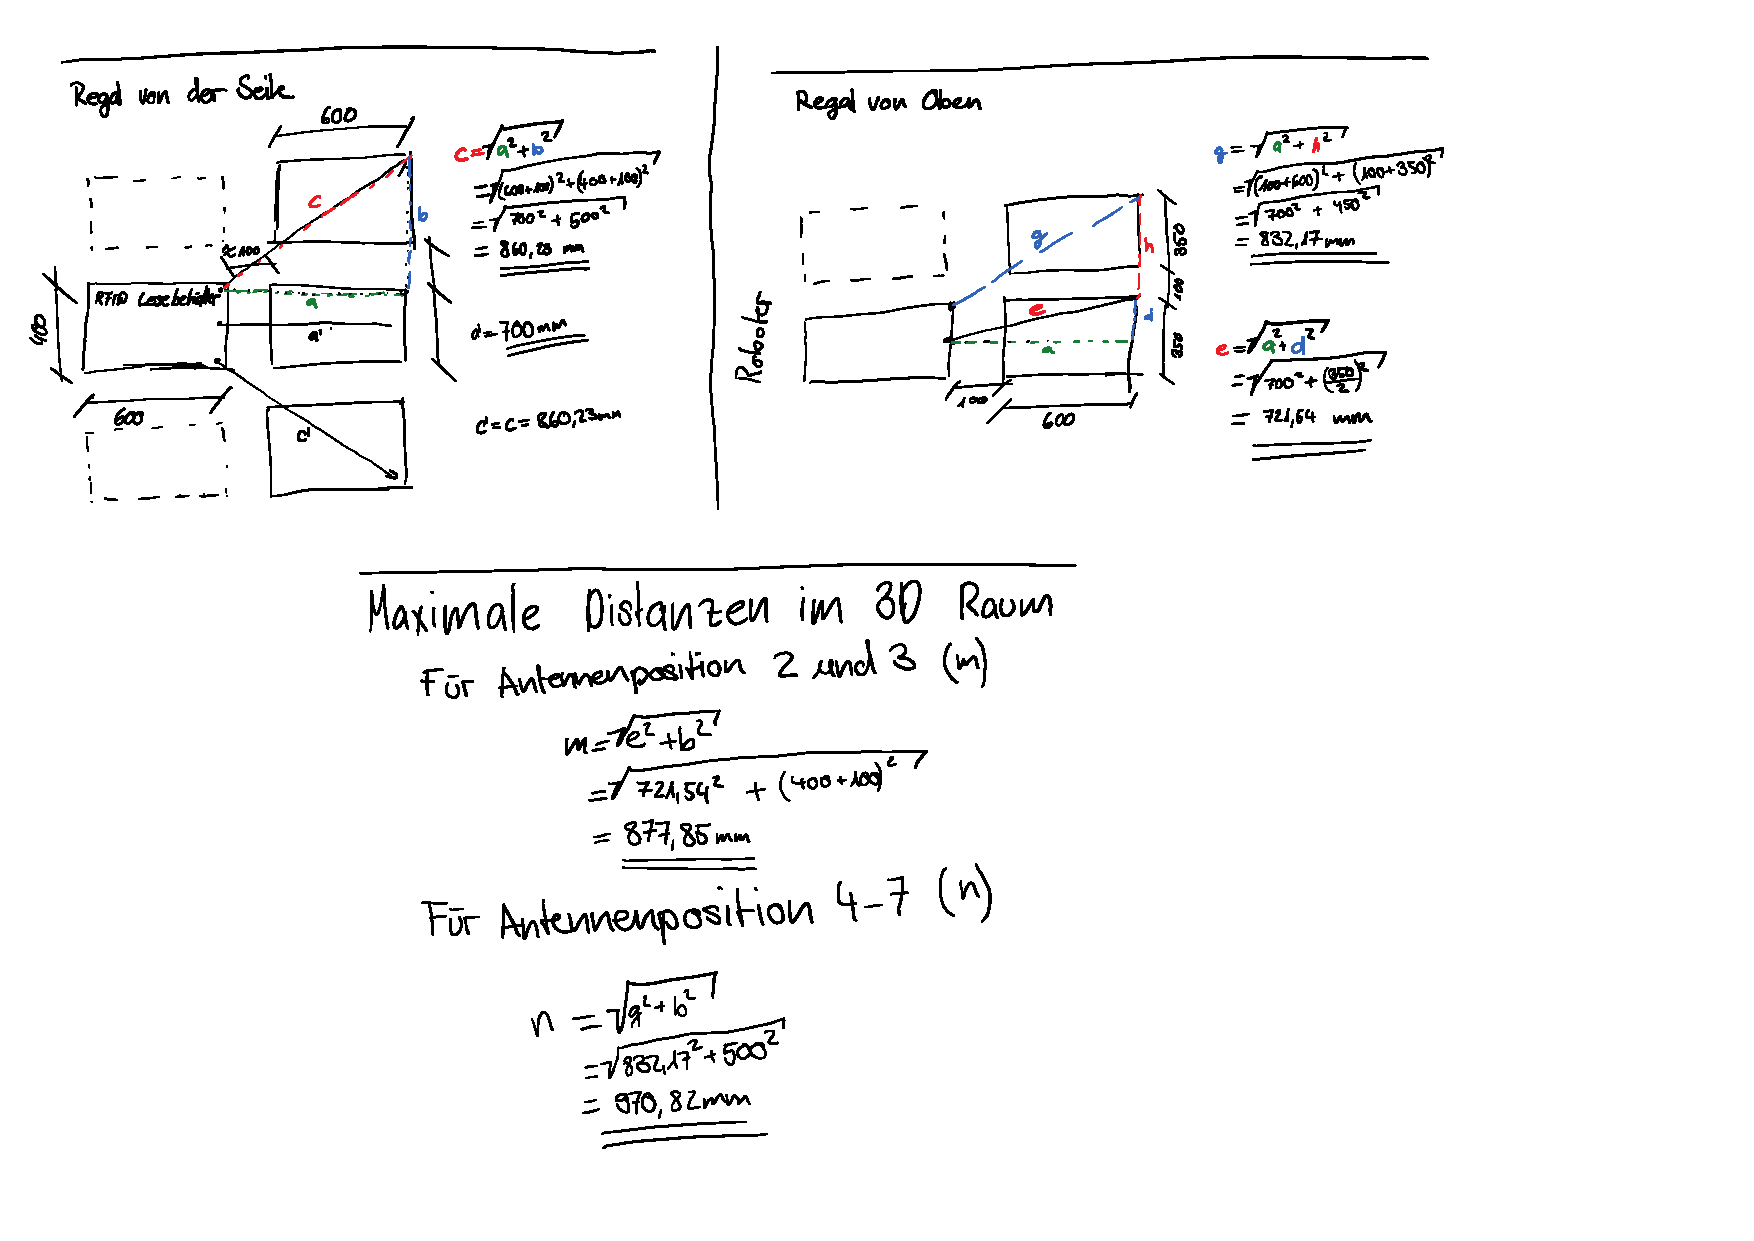
\includegraphics[keepaspectratio, width=1.2\textwidth]{berechnung_maximaler_distanz}
	\caption{Berechnung der maximalen Distanzen (alle Angaben in mm)}
	\label{fig:distanzcalc}
\end{figure}

Mangels Hersteller von RFID Lesegeräten, welche eine Lesereichweite von 1m oder mehr aufweisen, sollen folgende Komponenten von Feig Electronic verwendet werden. 
\begin{itemize}
	\item RFID Leser ID ISC.LR2500-A
	\item RFID Antennen ID ISC.ANT800/600
	\item RFID Antennenkabel ID ISC.ANT.C-A
	\item RFID 8xMultiplexer ID ISC.ANT.MUX
	\item Netzteil ID NET.24V-B
	\item Stromkabel ID CAB.NET.24V-B-EU
\end{itemize}

\clearpage
\subsection{Computer im Behälter}
Das RFID Lesegerät soll über einen kleinen, sich im Behälter befindenden Mini-Computer gesteuert werden. Dieser Computer soll über das bestehende WLAN Netzwerk auf die Datenbank zugreifen um die von RFID gescannten Behälter anhand der momentanen Position zu Identifizieren.  
Zudem soll die Fahrt des Roboter von diesem Minicomputer mittels den Anpassungen aus Kapitel  \ref{sec:roboterSWAnpassung} indirekt gesteuert werden.

Um diese Aufgabe zu übernehmen, soll ein Raspberry Pi verwendet werden.

\subsection{Kommunikation zum User}
Der User soll auf einem Stationären Computer über wichtige Informationen wie etwa die Dauer, den Fortschritt oder ob das zu suchende Exemplar bereits gefunden wurde informiert werden. Stationär bedeutet hier, dass es sich nicht um den Computer, welcher im Behälter ist, handelt.

\subsection{Stromzufuhr}
Für die komplette Stromversorgung soll ein Akku in dem Behälter verbaut werden, welcher genügend Kapazität für einen zehnstündigen Betrieb aufweist.

Der Stromverbrauch des RFID Lesers beträgt 35W bei 24V, das entspricht 1'458.32 mAh.
Der Stromverbrauch des Raspberry PI beträgt 4W bei 5V, das entspricht 800mAh.
Daher wird für eine Betriebsdauer von einer Stunde ein Akku mit einer Kapazität von mindestens 2'258.32 mAh benötigt. Um eine Betriebsdauer von zehn Stunden zu gewährleisten, benötigt der Akku eine Gesamtkapazität von mindestens 22'583.32 mAh.
Weiter hat er noch folgende Anforderungen.

\begin{itemize}
	\item USB Anschluss
	\item CH Wechselstromanschluss
	\item Geringes Gewicht
\end{itemize}

\subsection{Übersicht der Hardwarekomponenten}
Es sollen folgende Komponenten verwendet werden:

\begin{itemize}
	\item RFID Leser ID ISC.LR2500-A  (Feig)
	\item RFID Antennen ID ISC.ANT800/600 (Feig)
	\item RFID Antennenkabel ID ISC.ANT.C-A (Feig)
	\item Netzteil für Leser ID NET.24V-B (Feig)
	\item Netzkabel für Netzteil ID CAB.NET.24V-B-EU  (Feig)
	\item Minicomputer Raspberry PI 3 Model B + (Raspberry PI)
	\item USB-Kabel für Minicomputer Aukey CB-D11 (Aukey)
	\item Akku Goal Zero Yeti 400 Lithium (Goal Zero)
\end{itemize}

\section{Finanzierungsplan}

\subsection{Kosten}

\subsubsection{Lese-/Suchbehälter}
Die Einzelpreise von Feig sind gleichwertig zu einer Bestellung eines 100er Stapels und wurden von Euro in Schweizer Franken umgerechnet (Wechselkurs 1.14).

\begin{tabularx}{\textwidth}{|r|X|r|r|}
	\hline 
	\textbf{Menge} & \textbf{Produkt} & \textbf{Kosten(CHF)} & \textbf{Kosten gesamt(CHF)} \\
	\hline 
	1 & RFID Reader ID ISC.LR2500-A (Feig) & 1'200 & 1'200 \\ 
	\hline 
	2 & RFID Multiplexer 8-fach HF Multiplexer (Feig) & 500 & 1'000 \\ 
	\hline 
	14 & RFID Antennen ID ISC.ANT800/600 (Feig)& 760 & 10'640 \\
	\hline
	16 & RFID Antennenkabel ID ISC.ANT.C-A (Feig) & 20 & 320 \\
	\hline
	1 & Netzteil ID NET.24V-B (Feig) & 30 & 30 \\
	\hline
	1 & Netzkabel ID CAB.NET.24V-B-EU (Feig) & 4 & 4 \\
	\hline
	1 & Rapberry PI 3 Model B+ & 40 & 40 \\
	\hline
	1 & SB-Kabel für Minicomputer Aukey CB-D11 (Aukey) & 15 & 15 \\
	\hline
	1 & Akku Goal Zero Yeti 400 Lithium (Goal Zero) & 1'000 & 1'000 \\
	\hline
	1 & Behälter 986417 (Kaiserkraft) & 39 & 39 \\
	\hline
	& & & \textbf{14'288} \\
	\hline
\end{tabularx} 
\subsubsection{Umbau Roboter SW}
Basierend auf den Stundenkosten der Firma bbv Software Services AG wurde die folgende Approximation errechnet.
Die Stunden für die Umsetzung basieren auf Annahmen.

\begin{tabularx}{\textwidth}{|r|r|X|r|}
	\hline 
	\textbf{Stunden(h)} & \textbf{Lohn(CHF/h)} & \textbf{Beschrieb} & \textbf{Kosten gesamt(CHF)} \\
	\hline 
	50 & 180 & Umsetzung, sofern die Software die Befehle bereits über das Netztwerk entgegennimmt. & 9'000 \\
	\hline
	200 & 180 & Umsetzung, sofern die Software komplexere Anpassung benötigt & 36'000 \\
	\hline
	8 & 200 & Allgemeine RE und weitere Kosten & 1'600 \\
	\hline	
	& & & \textbf{10'600 bis 37'600} \\ 
	\hline
\end{tabularx}
\\
Die Gesamtkosten können also zwischen 10'600.- und 37'600.- schwanken. Wobei diese Werte auf zwei Approximationen beruhen, und somit für deren Einhalt nicht garantiert werden kann.

\subsubsection{Gesamt Rechnung}
\begin{tabularx}{\textwidth}{|X|r|}
	\hline
	\textbf{Beschreibung} & \textbf{Kosten (CHF)} \\
	\hline
	RFID Lese-/Suchbehälter & 14'288 \\
	\hline
	Umbau Roboter SW & 10'600 bis 37'600 \\
	\hline
	Weitere BDA für Implementation & 1'000 \\
	\hline
	& \textbf{25'888 bis 52'888} \\
	\hline
\end{tabularx}

\subsection{Kosten Manuelle Suche}
Würde ein Exemplar deplatziert werden, würde eine aufwendige Suche beginnen, welche bei etwa drei Millionen Exemplaren viel Zeit benötigt. Würde es theoretisch möglich sein ein Exemplar pro Sekunde zu durchsuchen bräuchte man etwa drei Millionen Sekunden. Dies entspricht 50'000 Minuten oder 833.32 Stunden oder 104.17 Arbeitstage à 8h oder knapp 5 Monaten. Würde diese Arbeit von einer Student*in mit einem Stundenlohn von etwa 20 CHF durchgeführt, könnte diese Suche bis zu 16'666.67 CHF kosten. Würde die Suche von einem Arbeiter der Speicherbibliothek übernommen werden, würden die Kosten noch höher ausfallen.

Die Kosten von 52'888 würden nach gut drei Suchvorgängen die Kosten der manuellen Suche eingeholt haben. Zusätzliche gäbe es einen Zeitgewinn von knapp 103 Arbeitstagen, da die Suche der Exemplare nach einem Tag abgeschlossen ist.
